% Landaur embedding is embedding functions inside a larger function that we can then uncall
% Allows for irreversibility but makes the computer more of a lookup table than an actual computer
% We get around this by only allowing logically reversible computations

% Bennet embedding is what we want to use?

\section{Embeddings and heat dissipation}
Another motivation for researching reversible computing is heat dissipation; current transitor-based computing devices dissipate energy as heat and cooling of computational devices has become the main focus for the semiconductor industry \cite{semiconductors_valley}. In 1961 R. Landaur suggested reversible computing could be a way to minimize energy dissipation from a system \cite{Irreversibility_paper}.
Similar to how kinetic and potential energy work, computing a result would put the machine in a state with some energy that would enable it to invert the computation.
Landaur also proposed a way to make irreversible programs reversible. We call this the Landaur embedding.
%Most languages are not reversible, because they throw away information about the computers history, making it ambigious to find the predecessor state. 

%Logic reversibility implies that information is conserved and most languages are not backwards deterministic because some of their operations are logically irreversible and throw away information about the computers history, making it ambiguous to find the predecessor state.
%Embeddings are a way to make an irreversible computer reversible.

\subsection{Landaur embedding}
What Landaur saw was that any logically irreversible program could be transformed into a reversible one by wrapping it in a larger program with extra parameters that could hold any information needed for reversability. He proposed that the computer could have an extra tape where it would save all of its computation history. That way it would know how to run in reverse. But the size of saving this computation history is proportional to the execution time of the program.

Based on the idea that computation is cheap and erasure of data is expensive, Landaur's Embedding is not very efficient since it merely postpones the inevitable erasure of information when the tape needs to be cleared before the next computation.
Landaur demonstrated that whenever a computer throws away information about its previous state it results in a heat dissipation of $kT ln 2$ for each bit of information lost.
\subsection{Bennett embedding}
In 1973 C.H. Bennett came up with a new embedding that would turn out to be much more useful\cite{Bennett1973LogicalRO}.
The idea is that the machine can use the inverse of its transition function to carry out the entire computation backwards, completely resetting the history tape to its original blank state by computation. One only needs to copy over the output once it has been calculated before starting the cleanup. This way the data is reset through computation instead of erasure, which in theory should be much cheaper.
It uses three tapes: one for the forwards/backwards calculation, one for computation history and a third for copying over the output. 
In theory, this reduces the energy dissipated by roughly a factor ten.

\section{Reversibility in Hermes}
% We do not overwrite data in Hermes until we have set it back to 0 at the end of the function?
Hermes is a reversible programming language designed for encryption algorithms. It offers forwards determinism as well as backwards determinism its calculations, meaning that nomatter if it executes forwards or backwards,  there is only one possible state that the machine can transition to nomatter what state it is currently in.
This results in a one-to-one relationship between input and output states that is achieved through reversible updates, swaps and so on.
% Hermes uses pass-by-reference, so no global variables.
Hermes and its predecessor Janus uses pass-by-reference, which is where every argument passed to a function is a direct reference to the variable.
This imposes certain restrictions on parameter passing: there has to be the same amount of parameters for a call / uncall of a function as these are implicitly both the input and output of a function.
There can be no global variables and no variable can be passed to a function multiple times e.g. \emph{foo(x, x, y)}.
Furthermore, an alias on both sides of an update such as \textbf{x += x / y} can break reversibility.

% Show Hermes grammar?
\subsection{Grammar}
The grammar of Hermes is as follows:
\begin{figure}[htp]
\centering
\begin{tabular}{>{$}l<{$}>{$}r<{$}>{$}l<{$}}
    Program   & \rightarrow & Procedure^+ \\[7pt]
    Procedure & \rightarrow & \textbf{id} \; ( \; Decls2^? \; ) \; Stmt \\[7pt]
    Stmt      & \rightarrow &; \\
              & |           & Lval \; \textbf{update} \; Exp \;; \\
              & |           & Lval\text{++} \;; \\
              & |           & Lval\text{- -} \;; \\
              & |           & \texttt{if} \; ( \; Exp \; ) \; Lval \; \textbf{update} \; Exp \;; \\
              & |           & Lval \; \text{<->} \; Lval \;; \\
              & |           & \texttt{if} \; ( \; Exp \; ) \; Lval \; \text{<->} \; Exp \;; \\
              & |           & \texttt{for} \; ( \; \textbf{id} = Exp \; ; \; Exp \; ) \; Stmt  \;; \\
              & |           & \texttt{assert} \; ( \; Exp \; ) \;; \\
              & |           & \texttt{call} \; \textbf{id} \; ( \; Lvals \; ) \;; \\
              & |           & \texttt{uncall} \; \textbf{id} \; ( \; Lvals \; ) \;; \\
              & |           & \texttt{printf} \; ( \; \textbf{stringConst} \; , \; Lvals \; ) \;; \\
              & |           & \texttt{scanf} \; ( \; \textbf{stringConst} \; , \; Lvals \; ) \;; \\
              & |           & \{ \; Decls1 \; Stmt^* \; \} \\[7pt]
    Exp       & \rightarrow & Lval \\
              & |           & \textbf{numConst} \; \\
              & |           & Exp \; \textbf{binOp} \; Exp \\
              & |           & \textbf{unOp} \; Exp \\
              & |           & ( \; Exp \; ) \; \\[7pt]
    Lval      & \rightarrow & \textbf{id}\\
              & |           & \textbf{id} \; [ \; Exp \; ] \\[7pt]
    Lvals     & \rightarrow & Lval \\
              & |           & Lval \; , \; Lvals \\[7pt]
    VarSpec   & \rightarrow & \textbf{id}\\
              & |           & \textbf{id} \; [ \; \textbf{numConst} \; ] \\[7pt]
    VarSpecs  & \rightarrow & VarSpec \\
              & |           & VarSpec \; , \; VarSpecs \\[7pt]
    Decls1    & \rightarrow & \\
              & |           & \textbf{type} \; Varspecs \; ; \; Decls1\\
              & |           & \texttt{const}\;\textbf{type}\;\textbf{id}\;=\textbf{numConst}\;;\;Decls1\;\\[7pt]
    Decls2    & \rightarrow & \textbf{type} \; VarSpec \\
              & |           &  \textbf{type} \; VarSpec \; , \; Decls2

\end{tabular}
\caption{Grammar of Hermes.}
\label{fig: grammar}
\end{figure}



% Show control flows?
\subsection{Control flows}
Unlike most other programming languages (including Janus), Hermes does not have branching. It has two special types of if-statements being the conditional update and conditional swap. These conditionals only allow for one line of code to be executed, i.e. the swap or the update, and have a constant execution time. This is because they are constructed in such a way that the code of the conditional is always evaluated but only takes effect or gets executed if the condition is true.
Conditionals work on integers, which with the help of a logical AND, allows the update to only update in cases where the conditional is non-zero, i.e. true. As seen from figure ~\ref{fig:conditionals_c}, the conditional \textbf{(0 != a < 2)} with a minus in front either returns 0 or -1, which as a signed bit-representation is all ones, meaning that whatever you AND will remain in the result. This makes the update take effect. Had the conditional been 0, the AND operation would have resulted in bits being 0, which would have turned the expression into \textbf{x += 0}.
Swap is done with three XOR operations, which ensures reversability and does not introduce any extra temporary variables.
\begin{figure}
    \centering
    \begin{minipage}{0.35\textwidth}
        \centering
        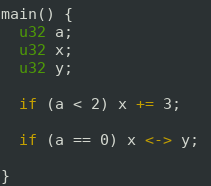
\includegraphics[width=0.9\textwidth]{conditionals_hms.png}
        \caption{Conditionals in Hermes}
    \end{minipage}\hfill
    \begin{minipage}{0.60\textwidth}
        \centering
        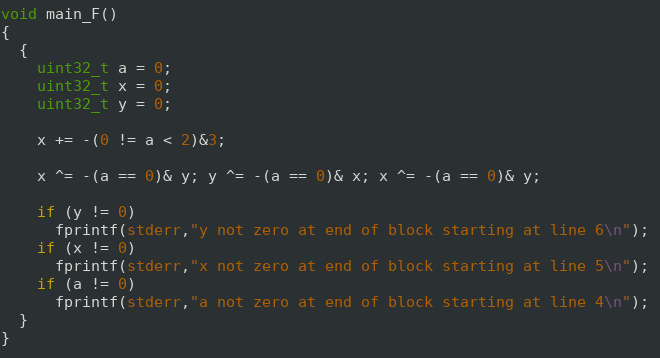
\includegraphics[width=0.9\textwidth]{conditionals_c.png}
        \caption{Conditionals translated to C}
        \label{fig:conditionals_c}
    \end{minipage}
\end{figure}

% Hermes has const arrays now
\subsection{Constants}
Hermes allows for constant values to be declared. These are not required to be 0 at the end of a function and are initialized with a value other than 0. However, it was only singleton values that were allowed to use the const keyword so I added the ability to specify constant arrays of varying sizes. This was done by adding an entry for it in the AST, the Compiler and the typesystem.
%(* TODO: I also added out of bounds checks *)

Being able to define const arrays is very useful for algorithms such as Twofish that have large 16x16 arrays. In the past, populating large arrays was done through a call to a function that would add values to all the entries of the array. Now it can be done directly in the function that uses it.
